\documentclass{article} % For LaTeX2e
\usepackage{nips14submit_e,times}
\usepackage{amsmath}
\usepackage{amsthm}
\usepackage{amssymb}
\usepackage{mathtools}
\usepackage{hyperref}
\usepackage{url}
\usepackage{algorithm}
\usepackage[noend]{algpseudocode}
%\documentstyle[nips14submit_09,times,art10]{article} % For LaTeX 2.09

\usepackage{graphicx}
\usepackage{caption}
\usepackage{subcaption}
\usepackage{tikz-cd}

\def\eQb#1\eQe{\begin{eqnarray*}#1\end{eqnarray*}}
\def\eQnb#1\eQne{\begin{eqnarray}#1\end{eqnarray}}
\providecommand{\e}[1]{\ensuremath{\times 10^{#1}}}
\providecommand{\pb}[0]{\pagebreak}
\DeclarePairedDelimiter\ceil{\lceil}{\rceil}
\DeclarePairedDelimiter\floor{\lfloor}{\rfloor}

\newcommand{\E}{\mathrm{E}}
\newcommand{\Var}{\mathrm{Var}}
\newcommand{\Cov}{\mathrm{Cov}}

\def\Qb#1\Qe{\begin{question}#1\end{question}}
\def\Sb#1\Se{\begin{solution}#1\end{solution}}

\newenvironment{claim}[1]{\par\noindent\underline{Claim:}\space#1}{}
\newtheoremstyle{quest}{\topsep}{\topsep}{}{}{\bfseries}{}{ }{\thmname{#1}\thmnote{ #3}.}
\theoremstyle{quest}
\newtheorem*{definition}{Definition}
\newtheorem*{theorem}{Theorem}
\newtheorem*{lemma}{Lemma}
\newtheorem*{question}{Question}
\newtheorem*{preposition}{Preposition}
\newtheorem*{exercise}{Exercise}
\newtheorem*{challengeproblem}{Challenge Problem}
\newtheorem*{solution}{Solution}
\newtheorem*{remark}{Remark}
\usepackage{verbatimbox}
\usepackage{listings}
\usepackage{mathrsfs}
\title{DiffGeoI: \\
Problem Set VI}


\author{
Youngduck Choi \\
CIMS \\
New York University\\
\texttt{yc1104@nyu.edu} \\
}


% The \author macro works with any number of authors. There are two commands
% used to separate the names and addresses of multiple authors: \And and \AND.
%
% Using \And between authors leaves it to \LaTeX{} to determine where to break
% the lines. Using \AND forces a linebreak at that point. So, if \LaTeX{}
% puts 3 of 4 authors names on the first line, and the last on the second
% line, try using \AND instead of \And before the third author name.

\newcommand{\fix}{\marginpar{FIX}}
\newcommand{\new}{\marginpar{NEW}}

\nipsfinalcopy % Uncomment for camera-ready version

\begin{document}


\maketitle

\begin{abstract}
This work contains solutions to the exercises of the problem set I.
\end{abstract}

\bigskip

\begin{question}[1]
\hfill
\begin{figure}[h!]
  \centering
    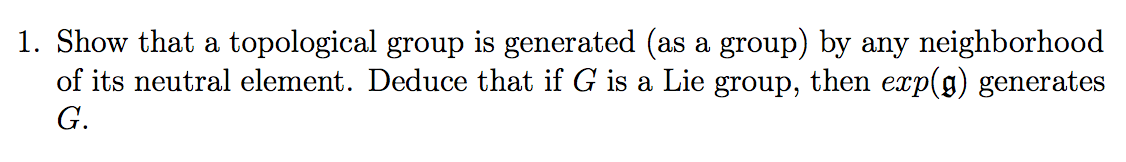
\includegraphics[width=0.7\textwidth]{DG-e6-p1.png}
\end{figure}
\end{question}
\begin{solution} \hfill \\
The first part of the problem should be corrected to a connected topological space.
Suppose $U$ is a neighborhood of $e$. Set
\eQb
U_n &=& \{ u_1...u_n \>\> | \>\> u_i \in U \>\>;\>\> \forall 1 \leq i \leq n\}
\eQe
for any $n \geq 1$, and $W = \cup_{n=1}^{\infty} U_n$.
For topological groups, $UV$ is open, if $U$ and $V$ are open, so
$U_n$ is open for all $n \geq 1$, which implies $W$ is open. At this point,
by connectivity of $G$, it suffices to show that $W$ is closed. Let $g \in \overline{
W}$. Then, as $gU^{-1}$ is an open neighborhood of $g$, there exists 
$h \in W \cap gU^{-1}$, so 
\eQb
h = gu^{-1} \>\>\> \text{and} \>\>\> h = u_1...u_n  
\eQe
for some $u \in U$, and $u_1,...,u_n \in U$, and hence
\eQb
g = u_1...u_n u \in U^{n+1} \subset W. 
\eQe
Therefore, $W$ is closed, and we are done. 

\bigskip

By property of $\exp$, 
\eQb
T_{e} \exp(v) = v 
\eQe
for any $v \in$ \textbf{g}. 
Therefore, $\exp$ is a local diffeomorphism at $e$, so 
$\exp( $\textbf{g}) contains a neighborhood of $e$. By (1), the result follows.

\hfill $\qed$ 

\end{solution}

\newpage

\begin{question}[2]
\hfill
\begin{figure}[h!]
  \centering
    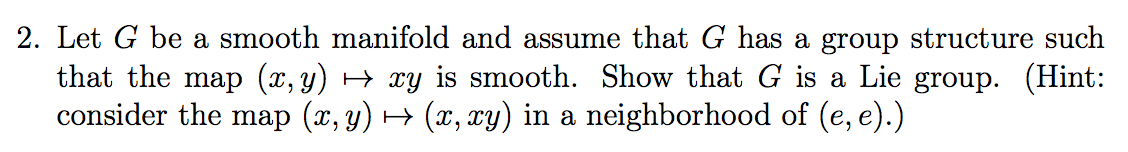
\includegraphics[width=0.7\textwidth]{DG-e6-p2.png}
\end{figure}
\end{question}
\begin{solution} \hfill \\
Set
\eQb
\triangle^{'} &=& \{ (g,g^{-1}) \in G \times G\}.
\eQe
As the multiplication map, $m$, 
is constant rank, surjective and smooth, it is a submersion.
Hence
\eQb
\triangle^{'} &=& m^{-1}(e) 
\eQe
is an embedded submanifold of $G\times G$ with dimension $n$. Let $\pi_1, 
\pi_2$ be standard projections of first, and second coordinates. Moreover,
$i$ be an inclusion map from $\triangle^{'} \to G \times G$, and 
$d:G \to \triangle^{'}$ be defined by $g \mapsto (g,g^{-1})$. Observe that
\eQb
\text{inv} = \pi_2 \circ i \circ d .
\eQe 
Therefore, it suffices to show that $d$ is smooth. Note that
\eQb
d &=& (\pi_1 \circ i)^{-1}. 
\eQe
Now, as $\pi_1 \circ i$ is a smooth bijection, where the differential is nonsingular
everywhere, by the inverse function theorem, $d$ is smooth, and we are done.
\hfill $\qed$


\end{solution}

\bigskip

\begin{question}[3]
\hfill
\begin{figure}[h!]
  \centering
    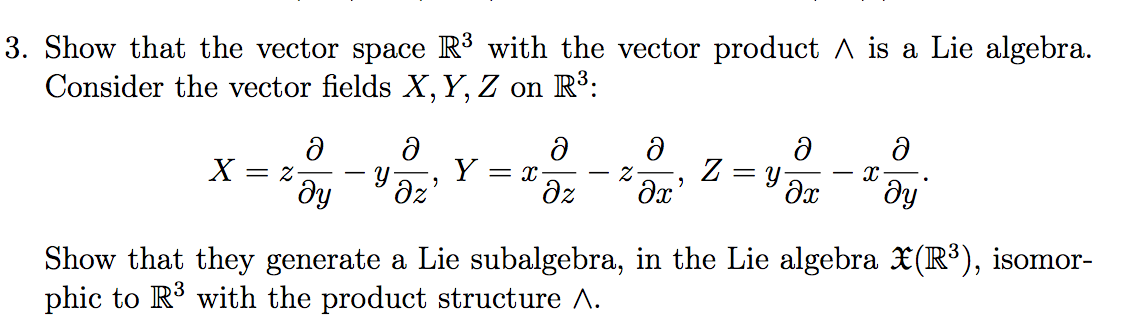
\includegraphics[width=0.7\textwidth]{DG-e6-p3.png}
\end{figure}
\end{question}
\begin{solution} \hfill \\
From ordinary calculus, we see that the cross product, when viewed as a binary
operation has bilinearity, alternativity and jacobi identity. Hence, it is a 
Lie-algebra on $\mathbb{R}^3$. 

\bigskip

We compute
\eQb
\left[ X,Y \right] 
&=& y \dfrac{\partial }{\partial x} - x\dfrac{\partial }{\partial y} = Z \\
\left[ X,Z \right]  &=&
 -x\dfrac{\partial }{\partial z} + z\dfrac{\partial }{\partial x} = -Y \\
\left[ Y,Z \right] &=&
 Z\dfrac{\partial }{\partial y} - y \dfrac{\partial }{\partial z} = X 
\eQe
and hence
\eQnb
[a_1 X + b_1 Y + c_1 Z, a_2 X + b_2 Y + c_2 Z] &=& 
(a_1b_2 - b_1 a_2)[X,Y] + (a_1 c_2 - c_1 a_2)[X,Z] \nonumber \\ 
&+& (b_1 c_2 - c_1 b_2)[Y,Z]  
\nonumber \\
&=&  (a_1b_2 - b_1 a_2)Z - (-a_1 c_2 - c_1 a_2)Y \nonumber \\
&+& (b_1 c_2 - c_1 b_2)X \label{eq:3.1} 
\eQne
for any $a_i, b_i, c_i$ with $i = 1,2$. The closure implies that 
$X, Y, Z$ generates a Lie subalgebra in $\mathscr{X}(\mathbb{R}^3)$ with $[,]$. 

\bigskip
Let $\Phi$ be the map that sends an element in the subalgebra to $\mathbb{R}^3$
by the coefficients of $X, Y , Z$ in order. If $X_1 = a_1 X + b_1 Y + c_1Z$
and $X_2 = a_2 X + b_2 Y + c_2 Z$, then, from~\eqref{eq:3.1},
\eQb
\Phi([X_1,X_2]) &=& (b_1c_2 - c_1b_2, -a_1c_2 + c_1a_2, a_1b_2 - b_1 a_2) \\ 
&=& (a_1,b_1,c_1) \wedge (a_2, b_2, c_2) = \Phi(X_1) \wedge \Phi(X_2). \\ 
\eQe
Hence, $\Phi$ is a Lie Algebra isomorphism. \hfill $\qed$
\end{solution}


\end{document}

